%!TEX root = Literature_Review_David_Burns.tex

%Todo

% - send to mum for editing
% - send to zoran to check content

%Done

% - Get rough version of totally complete chapter
% - remove all the '' reminders and any quotations
% - trim down some of these sections, just because you reviewed the paper intensely doesnt mean you need it all
% - put in self referencing
% - prep final draft


\chapter{Dimethyl Sulphide}
\label{ch:dms}

Dimethyl sulphide (\gls{dms}) is a naturally produced chemical that has been theorised to influence cloud coverage and potentially act as a negative feedback mechanism for climate change \citep{charlson:1987fw}. \gls{dms} enters the atmosphere and goes through an array of chemical reactions to produce sulphuric acid (\gls{h2so4}) \citep{barnes:2006ug}, which may then nucleate into aerosols that can act as \gls{ccn}. Measurements of aerosols in the atmosphere, particular remote marine areas show a large percentage being of the non-sea salt sulphate variety, potentially sourced from \gls{dms} \citep{o1997marine}.  

%--------------------------------------------------------------------------------------------------------------------------%
%--------------------------------------------------------------------------------------------------------------------------%

	\section{Chemistry}
	\label{sec:chem}

	The chemical processes that \gls{dms} and dimethyl sulfoxide \gls{dmso} undergo in the atmosphere are extremely complicated with many competing pathways (see \cref{fig:dmspath}). \citet{barnes:2006ug} have reviewed the extensive literature on this subject, with great detail. They split the problem into three sections, the first, \gls{dms} reactions and products, the second, \gls{dmso} reactions and products, and the third, multiphase chemistry of the \gls{dms} pathways.

	The reaction processes for \gls{dms} are reactions with the \gls{oh} radical, the \gls{no3} radical, and with Halogen Atoms and Oxides.  During the day the dominant reaction is the addition pathway through \gls{oh}, while at night it is the abstraction pathway through \gls{no3} as seen in \cref{fig:dmspath} \citep{barnes:2006ug}. Pathways involving halogen species are generally ignored in modelling due to low availability, though levels of hypobromite high enough to be influential have been measured in the troposphere \citep{platt2003role}.

	\begin{figure}[!htb]
	 	\centering
	    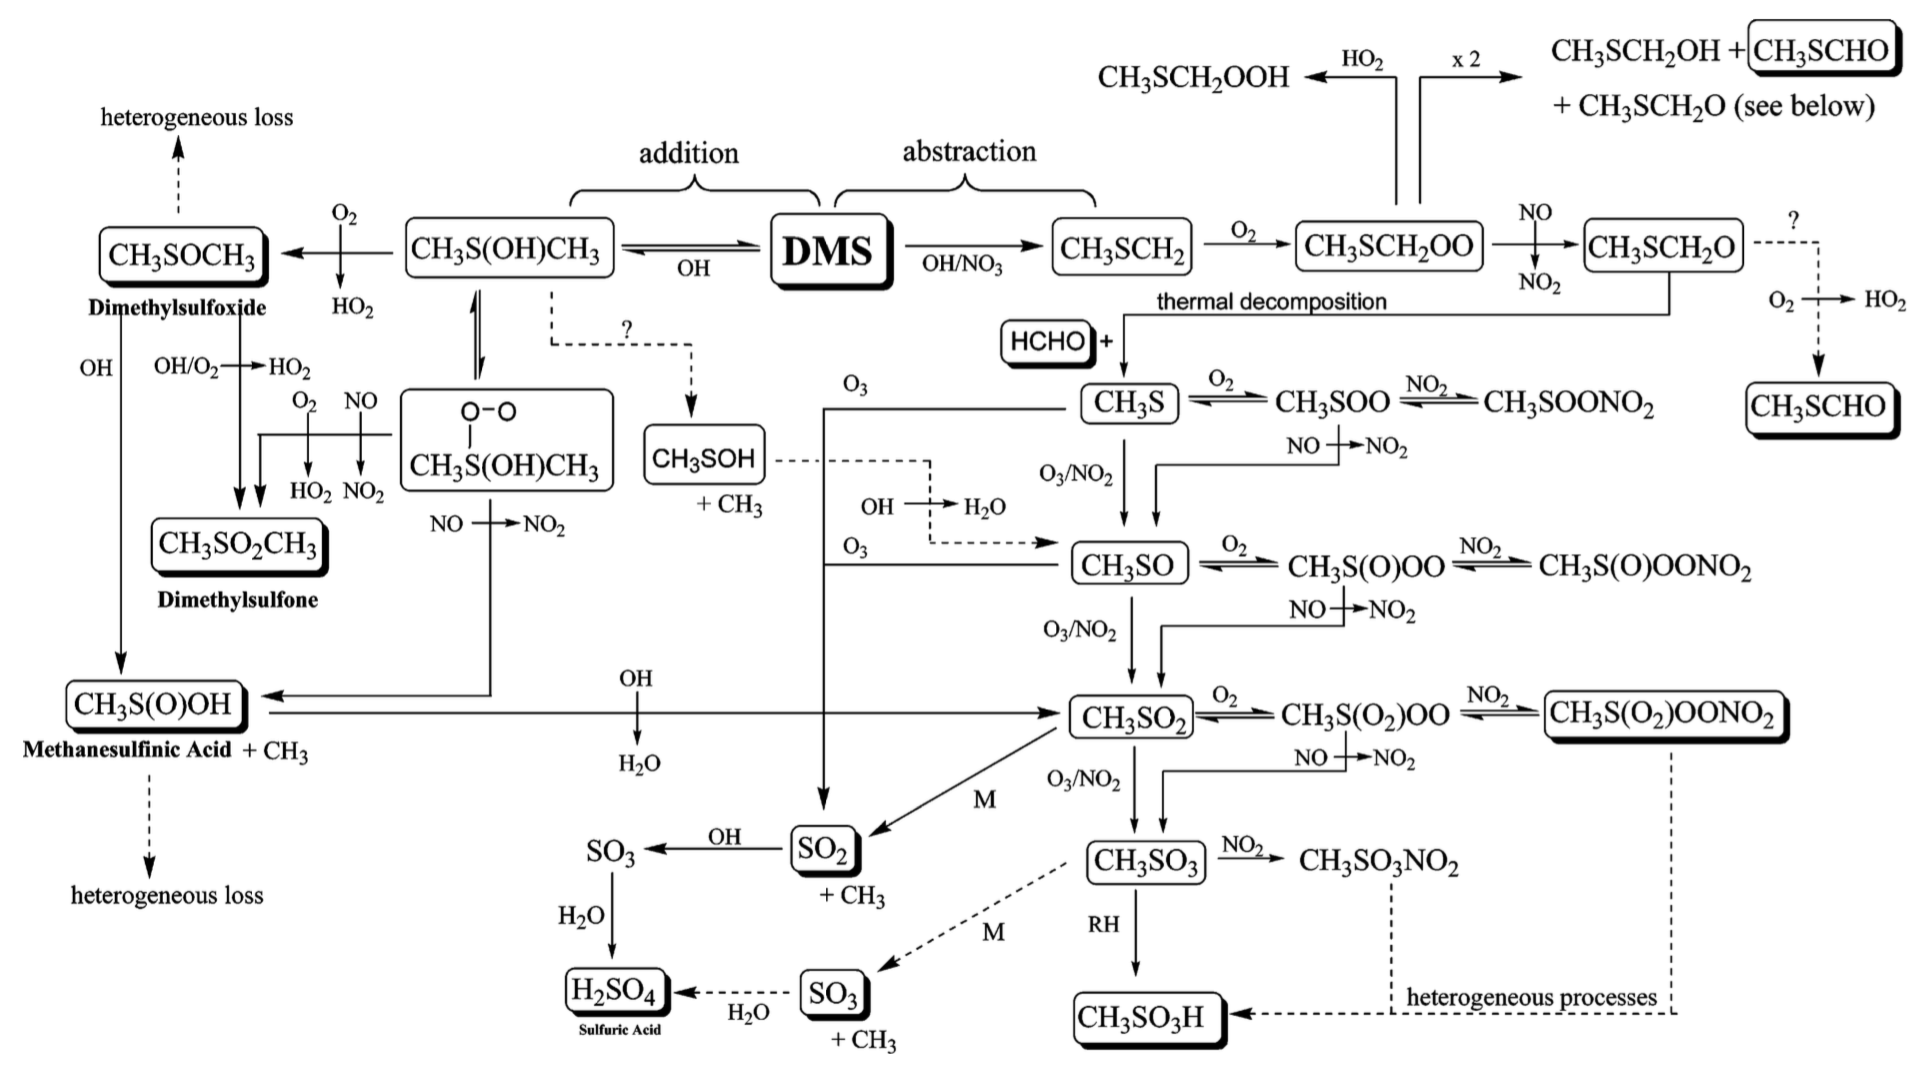
\includegraphics[width=0.95\textwidth,natwidth=1924,natheight=1068]{Fig/dms_Pathway.png}
	    \caption{The reaction scheme for \gls{dms} oxidised by \gls{no3} and \gls{oh} radicals \citep{barnes:2006ug}.}
	    \label{fig:dmspath}
	\end{figure}

	\gls{dmso} appears to be the major product of \gls{dms} oxidation in the atmosphere. Its reactions are the same as for \gls{dms} listed above. The atmospheric lifetimes calculated indicate that \gls{oh} radicals dominate reactions for \gls{dmso} \citep{barnes:2006ug}. Methane sulphinic acid (\gls{msia}) is a product of this reaction, which goes on to form methane sulphonic acid (\gls{msa}). \gls{dmsot} is also a product of this reaction and was considered the most prevalent pathway, but \citet{barnes:2006ug} found instead that the \gls{msia} pathway heavily dominates. \gls{sot} is the largest possible outcome of \gls{msa} oxidation.

	\subsection{Multiphase Chemistry}
	\label{subsec:multchem}

	The pathways examined in the preceding section are for gas phase reactions. However the atmosphere also contains liquid water in the form of droplets leading to aqueous phase reactions. The difference between gas and aqueous phase reactions is largely due to the availability of \gls{h2o} and \gls{hp} \citep{barnes:2006ug}. A combination of the two, multiphase chemistry, is needed. Interestingly, \gls{dms} is not as soluble in water as \gls{dmso}, \gls{dmsot}, \gls{msa} and \gls{msia} so its multiphase reactions are not as important.

	\citet{barnes:2006ug} have analysed the multiphase chemistry of all five chemicals and recommend that modellers implement the multiphase chemistry they have illustrated. They include a list of aqueous phase rate coefficients for the five chemicals of major interest, though do not consider a coupling of the gas and aqueous-phase systems necessary. \citet{jacob2000heterogeneous} provides a method for calculating chemical uptake by aerosols, while Henry's law is recommended for calculating concentrations, as an approximation.
	

%--------------------------------------------------------------------------------------------------------------------------%
%--------------------------------------------------------------------------------------------------------------------------%

	\section{Dimethyl Sulphide, Aerosols and the Environment}
	\label{sec:daande}


%--------------------------------------------------------------------------------------------------------------------------%

		\subsection{The CLAW Hypothesis}
		\label{subsec:clawhyp}

		\begin{figure}[!htb]
	 	    \centering
	 	    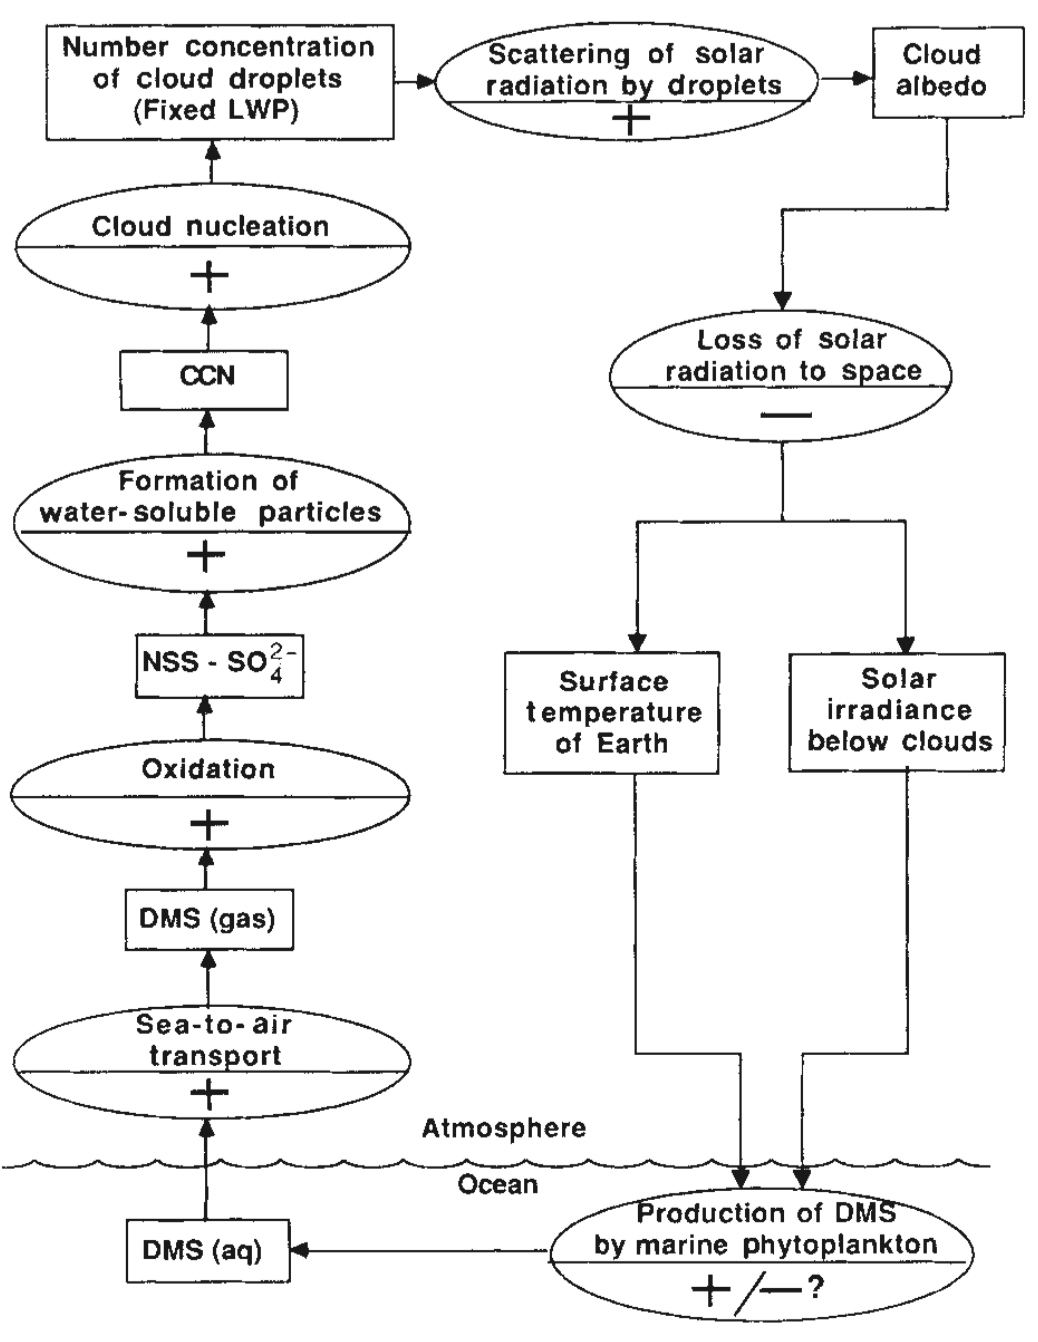
\includegraphics[width=0.7\textwidth,natwidth=1038,natheight=1342]{Fig/Original_Claw_Cycle.png}
	 	    \caption{The original feedback loop diagram describing the \gls{claw} hypothesis postulated in the paper by \citet{charlson:1987fw}. Rectangles are measurables, ovals are processes. The sign indicates the effect a positive change in the previous rectangle has on the next rectangle. The appearance of both signs in the production of \gls{dms} oval reflects the author's uncertainty of this particular effect. If it is positive, then the diagram describes a negative feedback loop, stabilising the climate.}
	 	    \label{fig:origclaw}
	 	\end{figure}

		In the \gls{claw} hypothesis \gls{dms} produced by phytoplankton in the ocean was considered as the precursor for \gls{ccn} in the \gls{mbl}. The \gls{ccn} produced were investigated for their cloud producing properties and the subsequent change in planetary albedo. The feedback loop, as seen in \cref{fig:origclaw}, was closed by linking the \gls{dms} precursor dimethylsulphoniopropionate (\gls{dmsp}) to a survival trait of the phytoplankton.

		Anthropogenic sources were ignored as the regions the hypothesis focussed on were remote, while other natural gaseous sulphur producers were considered insignificant. The purpose for phytoplankton's production of \gls{dms} was suggested to be from \gls{dmsp}, used in osmo-regulation and the cycle for methionine \citep{vairavamurthy:1985gw}. The highest flux of \gls{dms} from the ocean to the atmosphere was concluded to occur in the most saline, hottest and sunlit areas. The formation of sub-micrometer \gls{nss} sulphate particles was attributed to the oxidation of \gls{dms} by hydroxide. Other reactions removing \gls{dms} to non \gls{ccn} forms were considered too low to have a significant effect. From here it was concluded that increases in \gls{dms} flux from the ocean directly increased the number of \gls{ccn} present in the form of NSS sulphate aerosols \citep{charlson:1987fw}.

		\citet{charlson:1987fw} attempted to establish \gls{nss} sulphate as the prominent \gls{ccn} in the remote marine atmosphere and that higher concentrations increased or altered the reflective properties of cloud cover and thus albedo. \gls{nss} sulphate particles derived from \gls{dms} were considered to be in the right size range and have the correct properties for acting as \gls{ccn}. They used a model developed by \citet{twomey:1977} to predict the change in albedo from the change in the number of \gls{ccn}. By keeping the water content constant and increasing the number of \gls{ccn}, the mean radius of the droplets formed decreased. However the overall surface area of the droplets increased, thereby increasing cloud albedo. The model was used along with top of cloud satellite data to predict a change of $0.016$ to planetary albedo from a \SI{30}{\percent} increase in \gls{ccn}.

		The final part of the loop involved the \gls{dmsp} production mechanism and an attempt to link phytoplankton species that emit large amounts of \gls{dmsp} with increased survival. A number of possible explanations were put forward, such as increased ocean salinity during ice ages, as \gls{dmsp} protects against dessication. The resulting accidental formation of \gls{ccn} may have acted as a further survival mechanism. This completes the hypothesis that a negative feedback mechanism exists where increases in the Earth's temperature increases planetary albedo which then decreases the Earth's temperature \citep{charlson:1987fw}.

		%The \citet{Charlson:1987fw} paper helped to establish what is now known as Earth Systems Science, and much inter-disciplinary collaboration as the various aspects of the feedback mechanism lie in different areas of science.

		An analysis of aerosol data collected at Cape Grim in Tasmania was one of the first attempts to experimentally validate the \gls{claw} hypothesis \citep{ayers:1991gd}. \citet{ayers:1991gd} compared concentrations of methane sulphonic acid (\gls{msa}) and concentrations of \gls{ccn}. \gls{msa} was considered a relevant surrogate for \gls{dms} in the absence of long term \gls{dms} data. The results showed a correlation between \gls{msa} and \gls{ccn} concentrations along with seasonal dependence. Interestingly, there was a period during winter where \gls{msa} dropped close to zero while \gls{ccn} did not, indicating the presence of an unknown \gls{ccn} source. The relationship between \gls{msa} and \gls{ccn} was found to be non-linear. This experiment showed that the production of \gls{ccn} from phytoplankton aspect of the \gls{claw} hypothesis was at least plausible.


%--------------------------------------------------------------------------------------------------------------------------%

		\subsection{Post-CLAW Research}
		\label{subsec:postclaw}

		The \gls{claw} hypothesis has prompted a large amount of research and experimentation. \citet{quinn:2011iv} explored this research and formed the view that the hypothesis has been invalidated. The three core elements of the \gls{claw} hypothesis were identified as follows: a significant proportion of \gls{ccn} in the \gls{mbl} must be \gls{dms} derived, changes in \gls{dms} derived \gls{ccn} cause changes to cloud albedo, and \gls{dms} production is affected by ocean surface temperatures and solar radiation changes due to cloud albedo \citep{quinn:2011iv}. The final cycle proposed by \citet{quinn:2011iv} can be seen in \cref{fig:quinncyc}.

		\citet{quinn:2011iv} identified two primary \gls{ccn} competitors, sea salt particles and primary organic particles. A significant amount of \gls{mbl} \gls{ccn} were found to have a sea salt nucleus. Experiments where particles were heated past \SI{600}{\celsius} reported \SI{20}{\percent} refractory particles sourced at \SI{400}{\metre} across the Atlantic, and \SI{40}{\percent} aboard a research ship in the north-east Atlantic. Sea salt particles are likely to be the only refractory particles present \citep{o1993physicochemical}. Sea salt particles were also found to make up \SI{60}{\percent} of evaporated cloud droplets. The difference in these percentages is because sea salt particles act as \gls{ccn} at lower supersaturations \citep{tang1997thermodynamic}.

		Primary organic particles are aerosolised through the same mechanism as sea salt, but the constituents come from the detritus of organisms which collects on the ocean surface. The larger organic particles may break up in the atmosphere due to UV exposure or acidification. According to measurements recorded in the North Atlantic ocean, mass concentration of these particles increased during bloom periods \citep{o2004biogenically}. Organic particles (and sea salt) may also scavenge \gls{dms} products, which removes their effect on \gls{ccn} concentrations, if the scavenging particle was already acting as a \gls{ccn}. Due to the seasonal nature of primary organic particles, they may account for some of the seasonal relationship originally found by \citet{ayers:1991gd}, between \gls{dms} and \gls{ccn} concentrations.

		For the remaining \gls{dms} derived particles, direct nucleation of \gls{dms} products likely occurs at the top of clouds, in the \gls{ft}. Clouds remove existing particles in this region, which decreases the available surface area, and promotes homogeneous nucleation \citep{perry1994further}. Deep convective clouds also move \gls{dms} up into the \gls{ft} \citep{clarke1998particle}. The faster winds present in the \gls{ft} would move the particles away from the \gls{dms}'s origin, breaking the localisation required for the feedback loop. \citet{quinn:2011iv} argues that the majority of \gls{dms} derived particles present in the \gls{mbl} are from this process.

		\citet{cainey:2007jj} similarly identified three main ideas through which the feedback mechanisms of the \gls{claw} hypothesis have been diminished. These are: the effectiveness of \gls{dms} to become \gls{ccn}, the prevalence of sea salt particles in the \gls{ccn} size range, and the direct aerosolisation of organic particles from the ocean surface through bubble bursting.

		\begin{figure}[!htb]
	 	    \centering
	 	    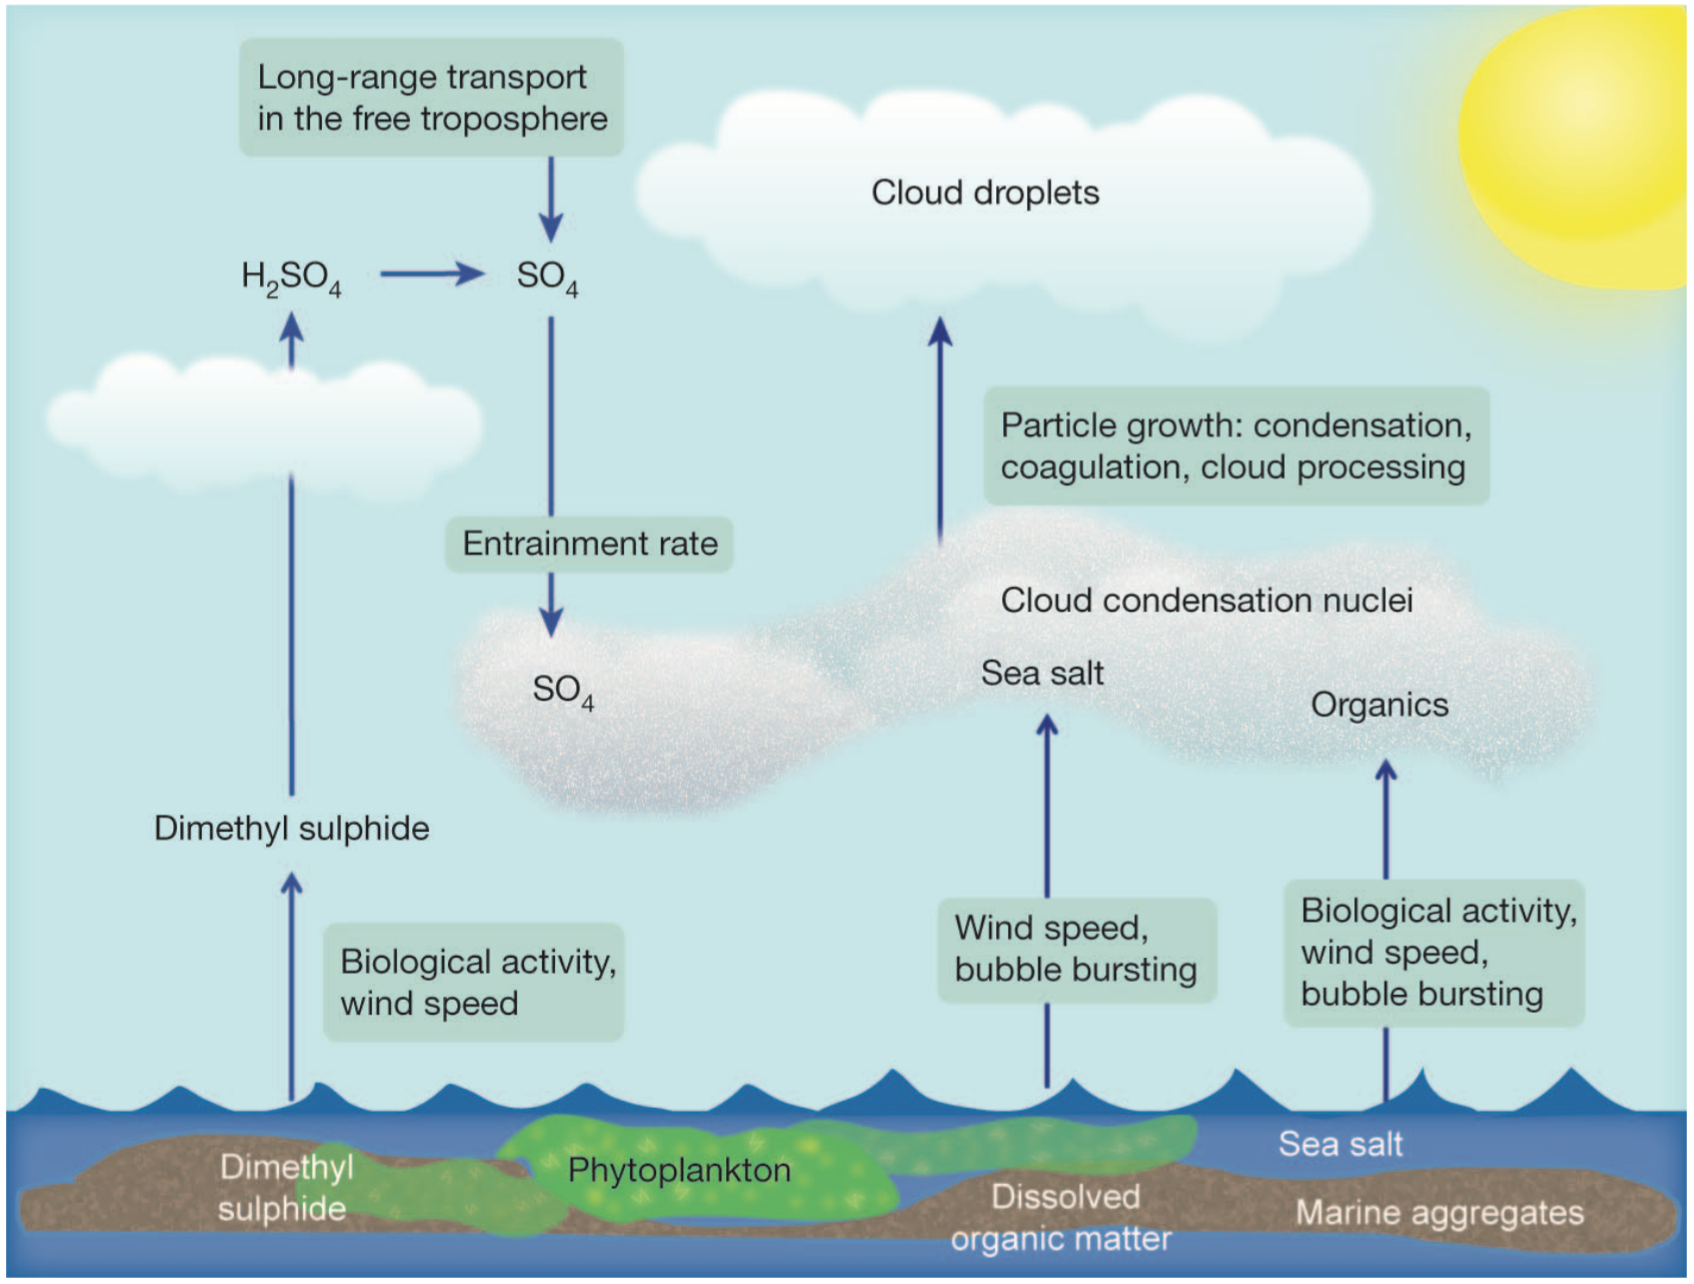
\includegraphics[width=0.8\textwidth,natwidth=1694,natheight=1284]{Fig/quinncycle.png}
	 	    \caption{An updated cycle for \gls{ccn} production in the \gls{mbl}. Major changes to the cycle in \cref{fig:origclaw} are nucleation in the \gls{ft} driven by clouds, and the presence of sea salt and primary organic aerosols \citep{quinn:2011iv}.}
	 	    \label{fig:quinncyc}
	 	\end{figure}

		The effect that aerosols have on cloud albedo is more complicated than the direct relationship proposed in the original \gls{claw} hypothesis \citep{quinn:2011iv, cainey:2007jj}. An increase in cloud albedo can be countered by a decrease in cloud fraction through improved entrainment of sub-saturated air around the cloud \citep{zuidema2008shortwave}. \citet{charlson:1987fw} predicted a \SI{1.3}{\celsius} decrease in surface temperature for a \SI{30}{\percent} increase in \gls{ccn}. As the extra \gls{ccn} are unlikely to be entirely \gls{dms} derived, the required increase in \gls{dms} flux would need to be very high, around \SI{300}{\percent} according to values modelled by \citet{woodhouse:2010ed}.

		An alternative action through which \gls{dms} derived sulphur compounds are removed, and thus prevented from becoming \gls{ccn} directly, is through heterogeneous nucleation onto existing particles \citep{cainey:2007jj}. Such an action may work to alter the chemistry of the particle and thus the albedo of the clouds formed from them. This may provide an alternate way for \gls{dms} to affect climate. 

		\citet{quinn:2011iv} advise that the \gls{claw} hypothesis should be retired, but acknowledge its impact in developing this area of science. Other mechanisms of climate regulation may still be present, such as sea salt particle concentration increases with wind speed, and primary organic particles with biological production. \citet{cainey:2007jj} take a more compromising stance, advising that research into the \gls{claw} hypothesis is still on-going and current results need to be fully implemented in modelling.


%--------------------------------------------------------------------------------------------------------------------------%
%--------------------------------------------------------------------------------------------------------------------------%
%Zoran said to remove :)
% \section{Links to experimentation 'rename'}

% 'do i even need this section?'

% how do you actually measure DMS or SO2? gas chromotography?
% From seawater collected.
% "DMS was trapped on a gold tube attached to the top of the purge chamber. These tubes were sealed with parafilm, labelled and analysed by gas chromatography for DMS at the laboratory (Curran et al. 1998)"
% \citep{Jones:2005ez}

% What is gas chromotography?

% What is pmf?
% Mark at CSIRO spoke about a technique called positive matrix factorisation which can give an estimate of a single chemical or aerosols source fractions. Write a bit about it in here.

% Matt said there is a website containing up to date chemical reaction rates in the atmosphere. Have a look at it and supply a list of the ones we are interested here.

% Experimentation can go either way with this model, and should probably have both. There are some things that we need measured to make the inputs of the model more accurate, particularly DMS surface flux around the \gls{gbr}. So establish a number of parameters that you think the model may predict, that can be checked with experimentation. Then list a number of paramaters that you would want tested to use as inputs for future runs of the model. Maybe even create a flow diagram of the modelling <-> experimentation structure.

